\documentclass[1p]{elsarticle_modified}
%\bibliographystyle{elsarticle-num}

%\usepackage[colorlinks]{hyperref}
%\usepackage{abbrmath_seonhwa} %\Abb, \Ascr, \Acal ,\Abf, \Afrak
\usepackage{amsfonts}
\usepackage{amssymb}
\usepackage{amsmath}
\usepackage{amsthm}
\usepackage{scalefnt}
\usepackage{amsbsy}
\usepackage{kotex}
\usepackage{caption}
\usepackage{subfig}
\usepackage{color}
\usepackage{graphicx}
\usepackage{xcolor} %% white, black, red, green, blue, cyan, magenta, yellow
\usepackage{float}
\usepackage{setspace}
\usepackage{hyperref}

\usepackage{tikz}
\usetikzlibrary{arrows}

\usepackage{multirow}
\usepackage{array} % fixed length table
\usepackage{hhline}

%%%%%%%%%%%%%%%%%%%%%
\makeatletter
\renewcommand*\env@matrix[1][\arraystretch]{%
	\edef\arraystretch{#1}%
	\hskip -\arraycolsep
	\let\@ifnextchar\new@ifnextchar
	\array{*\c@MaxMatrixCols c}}
\makeatother %https://tex.stackexchange.com/questions/14071/how-can-i-increase-the-line-spacing-in-a-matrix
%%%%%%%%%%%%%%%

\usepackage[normalem]{ulem}

\newcommand{\msout}[1]{\ifmmode\text{\sout{\ensuremath{#1}}}\else\sout{#1}\fi}
%SOURCE: \msout is \stkout macro in https://tex.stackexchange.com/questions/20609/strikeout-in-math-mode

\newcommand{\cancel}[1]{
	\ifmmode
	{\color{red}\msout{#1}}
	\else
	{\color{red}\sout{#1}}
	\fi
}

\newcommand{\add}[1]{
	{\color{blue}\uwave{#1}}
}

\newcommand{\replace}[2]{
	\ifmmode
	{\color{red}\msout{#1}}{\color{blue}\uwave{#2}}
	\else
	{\color{red}\sout{#1}}{\color{blue}\uwave{#2}}
	\fi
}

\newcommand{\Sol}{\mathcal{S}} %segment
\newcommand{\D}{D} %diagram
\newcommand{\A}{\mathcal{A}} %arc


%%%%%%%%%%%%%%%%%%%%%%%%%%%%%5 test

\def\sl{\operatorname{\textup{SL}}(2,\Cbb)}
\def\psl{\operatorname{\textup{PSL}}(2,\Cbb)}
\def\quan{\mkern 1mu \triangleright \mkern 1mu}

\theoremstyle{definition}
\newtheorem{thm}{Theorem}[section]
\newtheorem{prop}[thm]{Proposition}
\newtheorem{lem}[thm]{Lemma}
\newtheorem{ques}[thm]{Question}
\newtheorem{cor}[thm]{Corollary}
\newtheorem{defn}[thm]{Definition}
\newtheorem{exam}[thm]{Example}
\newtheorem{rmk}[thm]{Remark}
\newtheorem{alg}[thm]{Algorithm}

\newcommand{\I}{\sqrt{-1}}
\begin{document}

%\begin{frontmatter}
%
%\title{Boundary parabolic representations of knots up to 8 crossings}
%
%%% Group authors per affiliation:
%\author{Yunhi Cho} 
%\address{Department of Mathematics, University of Seoul, Seoul, Korea}
%\ead{yhcho@uos.ac.kr}
%
%
%\author{Seonhwa Kim} %\fnref{s_kim}}
%\address{Center for Geometry and Physics, Institute for Basic Science, Pohang, 37673, Korea}
%\ead{ryeona17@ibs.re.kr}
%
%\author{Hyuk Kim}
%\address{Department of Mathematical Sciences, Seoul National University, Seoul 08826, Korea}
%\ead{hyukkim@snu.ac.kr}
%
%\author{Seokbeom Yoon}
%\address{Department of Mathematical Sciences, Seoul National University, Seoul, 08826,  Korea}
%\ead{sbyoon15@snu.ac.kr}
%
%\begin{abstract}
%We find all boundary parabolic representation of knots up to 8 crossings.
%
%\end{abstract}
%\begin{keyword}
%    \MSC[2010] 57M25 
%\end{keyword}
%
%\end{frontmatter}

%\linenumbers
%\tableofcontents
%
\newcommand\colored[1]{\textcolor{white}{\rule[-0.35ex]{0.8em}{1.4ex}}\kern-0.8em\color{red} #1}%
%\newcommand\colored[1]{\textcolor{white}{ #1}\kern-2.17ex	\textcolor{white}{ #1}\kern-1.81ex	\textcolor{white}{ #1}\kern-2.15ex\color{red}#1	}

{\Large $\underline{12n_{0249}~(K12n_{0249})}$}

\setlength{\tabcolsep}{10pt}
\renewcommand{\arraystretch}{1.6}
\vspace{1cm}\begin{tabular}{m{100pt}>{\centering\arraybackslash}m{274pt}}
\multirow{5}{120pt}{
	\centering
	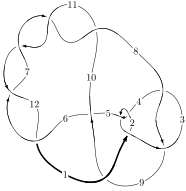
\includegraphics[width=112pt]{../../../GIT/diagram.site/Diagrams/png/2338_12n_0249.png}\\
\ \ \ A knot diagram\footnotemark}&
\allowdisplaybreaks
\textbf{Linearized knot diagam} \\
\cline{2-2}
 &
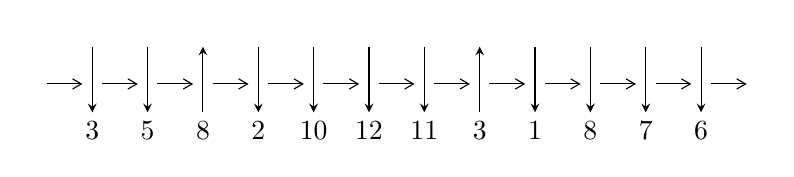
\begin{tikzpicture}[x=20pt, y=17pt]
	% nodes
	\node (C0) at (0, 0) {};
	\node (C1) at (1, 0) {};
	\node (C1U) at (1, +1) {};
	\node (C1D) at (1, -1) {3};

	\node (C2) at (2, 0) {};
	\node (C2U) at (2, +1) {};
	\node (C2D) at (2, -1) {5};

	\node (C3) at (3, 0) {};
	\node (C3U) at (3, +1) {};
	\node (C3D) at (3, -1) {8};

	\node (C4) at (4, 0) {};
	\node (C4U) at (4, +1) {};
	\node (C4D) at (4, -1) {2};

	\node (C5) at (5, 0) {};
	\node (C5U) at (5, +1) {};
	\node (C5D) at (5, -1) {10};

	\node (C6) at (6, 0) {};
	\node (C6U) at (6, +1) {};
	\node (C6D) at (6, -1) {12};

	\node (C7) at (7, 0) {};
	\node (C7U) at (7, +1) {};
	\node (C7D) at (7, -1) {11};

	\node (C8) at (8, 0) {};
	\node (C8U) at (8, +1) {};
	\node (C8D) at (8, -1) {3};

	\node (C9) at (9, 0) {};
	\node (C9U) at (9, +1) {};
	\node (C9D) at (9, -1) {1};

	\node (C10) at (10, 0) {};
	\node (C10U) at (10, +1) {};
	\node (C10D) at (10, -1) {8};

	\node (C11) at (11, 0) {};
	\node (C11U) at (11, +1) {};
	\node (C11D) at (11, -1) {7};

	\node (C12) at (12, 0) {};
	\node (C12U) at (12, +1) {};
	\node (C12D) at (12, -1) {6};
	\node (C13) at (13, 0) {};

	% arrows
	\draw[->,>={angle 60}]
	(C0) edge (C1) (C1) edge (C2) (C2) edge (C3) (C3) edge (C4) (C4) edge (C5) (C5) edge (C6) (C6) edge (C7) (C7) edge (C8) (C8) edge (C9) (C9) edge (C10) (C10) edge (C11) (C11) edge (C12) (C12) edge (C13) ;	\draw[->,>=stealth]
	(C1U) edge (C1D) (C2U) edge (C2D) (C3D) edge (C3U) (C4U) edge (C4D) (C5U) edge (C5D) (C6U) edge (C6D) (C7U) edge (C7D) (C8D) edge (C8U) (C9U) edge (C9D) (C10U) edge (C10D) (C11U) edge (C11D) (C12U) edge (C12D) ;
	\end{tikzpicture} \\
\hhline{~~} \\& 
\textbf{Solving Sequence} \\ \cline{2-2} 
 &
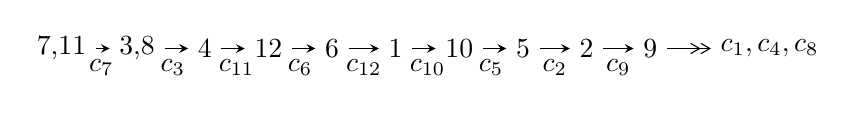
\begin{tikzpicture}[x=23pt, y=7pt]
	% node
	\node (A0) at (-1/8, 0) {7,11};
	\node (A1) at (17/16, 0) {3,8};
	\node (A2) at (17/8, 0) {4};
	\node (A3) at (25/8, 0) {12};
	\node (A4) at (33/8, 0) {6};
	\node (A5) at (41/8, 0) {1};
	\node (A6) at (49/8, 0) {10};
	\node (A7) at (57/8, 0) {5};
	\node (A8) at (65/8, 0) {2};
	\node (A9) at (73/8, 0) {9};
	\node (C1) at (1/2, -1) {$c_{7}$};
	\node (C2) at (13/8, -1) {$c_{3}$};
	\node (C3) at (21/8, -1) {$c_{11}$};
	\node (C4) at (29/8, -1) {$c_{6}$};
	\node (C5) at (37/8, -1) {$c_{12}$};
	\node (C6) at (45/8, -1) {$c_{10}$};
	\node (C7) at (53/8, -1) {$c_{5}$};
	\node (C8) at (61/8, -1) {$c_{2}$};
	\node (C9) at (69/8, -1) {$c_{9}$};
	\node (A10) at (11, 0) {$c_{1},c_{4},c_{8}$};

	% edge
	\draw[->,>=stealth]	
	(A0) edge (A1) (A1) edge (A2) (A2) edge (A3) (A3) edge (A4) (A4) edge (A5) (A5) edge (A6) (A6) edge (A7) (A7) edge (A8) (A8) edge (A9) ;
	\draw[->>,>={angle 60}]	
	(A9) edge (A10);
\end{tikzpicture} \\ 

\end{tabular} \\

\footnotetext{
The image of knot diagram is generated by the software ``\textbf{Draw programme}" developed by Andrew Bartholomew(\url{http://www.layer8.co.uk/maths/draw/index.htm\#Running-draw}), where we modified some parts for our purpose(\url{https://github.com/CATsTAILs/LinksPainter}).
}\phantom \\ \newline 
\centering \textbf{Ideals for irreducible components\footnotemark of $X_{\text{par}}$} 
 
\begin{align*}
I^u_{1}&=\langle 
u^{25}+2 u^{24}+\cdots+b-1,\;u^{27}+2 u^{26}+\cdots+a-2,\;u^{28}+2 u^{27}+\cdots-3 u-1\rangle \\
I^u_{2}&=\langle 
- u^3+u^2+b-2 u+1,\;u^4+3 u^2+a+1,\;u^5- u^4+4 u^3-3 u^2+3 u-1\rangle \\
\\
\end{align*}
\raggedright * 2 irreducible components of $\dim_{\mathbb{C}}=0$, with total 33 representations.\\
\footnotetext{All coefficients of polynomials are rational numbers. But the coefficients are sometimes approximated in decimal forms when there is not enough margin.}
\newpage
\renewcommand{\arraystretch}{1}
\centering \section*{I. $I^u_{1}= \langle u^{25}+2 u^{24}+\cdots+b-1,\;u^{27}+2 u^{26}+\cdots+a-2,\;u^{28}+2 u^{27}+\cdots-3 u-1 \rangle$}
\flushleft \textbf{(i) Arc colorings}\\
\begin{tabular}{m{7pt} m{180pt} m{7pt} m{180pt} }
\flushright $a_{7}=$&$\begin{pmatrix}1\\0\end{pmatrix}$ \\
\flushright $a_{11}=$&$\begin{pmatrix}0\\u\end{pmatrix}$ \\
\flushright $a_{3}=$&$\begin{pmatrix}- u^{27}-2 u^{26}+\cdots-4 u+2\\- u^{25}-2 u^{24}+\cdots+u+1\end{pmatrix}$ \\
\flushright $a_{8}=$&$\begin{pmatrix}1\\u^2\end{pmatrix}$ \\
\flushright $a_{4}=$&$\begin{pmatrix}-2 u^{27}-4 u^{26}+\cdots-2 u+3\\u^{27}+2 u^{26}+\cdots-3 u^2+1\end{pmatrix}$ \\
\flushright $a_{12}=$&$\begin{pmatrix}- u\\u\end{pmatrix}$ \\
\flushright $a_{6}=$&$\begin{pmatrix}u^2+1\\- u^2\end{pmatrix}$ \\
\flushright $a_{1}=$&$\begin{pmatrix}- u^3-2 u\\u^3+u\end{pmatrix}$ \\
\flushright $a_{10}=$&$\begin{pmatrix}u\\u^3+u\end{pmatrix}$ \\
\flushright $a_{5}=$&$\begin{pmatrix}- u^6-3 u^4+1\\- u^8-4 u^6-4 u^4-2 u^2\end{pmatrix}$ \\
\flushright $a_{2}=$&$\begin{pmatrix}- u^{27}- u^{26}+\cdots-6 u+2\\- u^{26}-2 u^{25}+\cdots+2 u+1\end{pmatrix}$ \\
\flushright $a_{9}=$&$\begin{pmatrix}u^9+6 u^7+11 u^5+6 u^3+u\\- u^9-5 u^7-7 u^5-2 u^3+u\end{pmatrix}$\\&\end{tabular}
\flushleft \textbf{(ii) Obstruction class $= -1$}\\~\\
\flushleft \textbf{(iii) Cusp Shapes $= - u^{27}-2 u^{26}-21 u^{25}-38 u^{24}-192 u^{23}-314 u^{22}-1007 u^{21}-1483 u^{20}-3363 u^{19}-4430 u^{18}-7513 u^{17}-8756 u^{16}-11482 u^{15}-11630 u^{14}-12024 u^{13}-10257 u^{12}-8392 u^{11}-5658 u^{10}-3552 u^9-1590 u^8-624 u^7+24 u^6+115 u^5+133 u^4+47 u^3+22 u^2-3 u-2$}\\~\\
\newpage\renewcommand{\arraystretch}{1}
\flushleft \textbf{(iv) u-Polynomials at the component}\newline \\
\begin{tabular}{m{50pt}|m{274pt}}
Crossings & \hspace{64pt}u-Polynomials at each crossing \\
\hline $$\begin{aligned}c_{1}\end{aligned}$$&$\begin{aligned}
&u^{28}+6 u^{27}+\cdots+17 u+1
\end{aligned}$\\
\hline $$\begin{aligned}c_{2},c_{4}\end{aligned}$$&$\begin{aligned}
&u^{28}-6 u^{27}+\cdots+5 u-1
\end{aligned}$\\
\hline $$\begin{aligned}c_{3},c_{8}\end{aligned}$$&$\begin{aligned}
&u^{28}+u^{27}+\cdots+96 u+32
\end{aligned}$\\
\hline $$\begin{aligned}c_{5}\end{aligned}$$&$\begin{aligned}
&u^{28}-2 u^{27}+\cdots+331 u-445
\end{aligned}$\\
\hline $$\begin{aligned}c_{6},c_{7},c_{10}\\c_{11},c_{12}\end{aligned}$$&$\begin{aligned}
&u^{28}-2 u^{27}+\cdots+3 u-1
\end{aligned}$\\
\hline $$\begin{aligned}c_{9}\end{aligned}$$&$\begin{aligned}
&u^{28}+2 u^{27}+\cdots+5 u+1
\end{aligned}$\\
\hline
\end{tabular}\\~\\
\newpage\renewcommand{\arraystretch}{1}
\flushleft \textbf{(v) Riley Polynomials at the component}\newline \\
\begin{tabular}{m{50pt}|m{274pt}}
Crossings & \hspace{64pt}Riley Polynomials at each crossing \\
\hline $$\begin{aligned}c_{1}\end{aligned}$$&$\begin{aligned}
&y^{28}+38 y^{27}+\cdots-17 y+1
\end{aligned}$\\
\hline $$\begin{aligned}c_{2},c_{4}\end{aligned}$$&$\begin{aligned}
&y^{28}-6 y^{27}+\cdots-17 y+1
\end{aligned}$\\
\hline $$\begin{aligned}c_{3},c_{8}\end{aligned}$$&$\begin{aligned}
&y^{28}-33 y^{27}+\cdots-14848 y+1024
\end{aligned}$\\
\hline $$\begin{aligned}c_{5}\end{aligned}$$&$\begin{aligned}
&y^{28}+22 y^{27}+\cdots-315151 y+198025
\end{aligned}$\\
\hline $$\begin{aligned}c_{6},c_{7},c_{10}\\c_{11},c_{12}\end{aligned}$$&$\begin{aligned}
&y^{28}+38 y^{27}+\cdots-15 y+1
\end{aligned}$\\
\hline $$\begin{aligned}c_{9}\end{aligned}$$&$\begin{aligned}
&y^{28}+34 y^{27}+\cdots-15 y+1
\end{aligned}$\\
\hline
\end{tabular}\\~\\
\newpage\flushleft \textbf{(vi) Complex Volumes and Cusp Shapes}
$$\begin{array}{c|c|c}  
\text{Solutions to }I^u_{1}& \I (\text{vol} + \sqrt{-1}CS) & \text{Cusp shape}\\
 \hline 
\begin{aligned}
u &= \phantom{-}0.152944 + 1.016320 I \\
a &= \phantom{-}1.019950 - 0.193834 I \\
b &= -0.647472 - 0.451263 I\end{aligned}
 & \phantom{-}3.33821 - 2.49897 I & -1.28357 + 4.65842 I \\ \hline\begin{aligned}
u &= \phantom{-}0.152944 - 1.016320 I \\
a &= \phantom{-}1.019950 + 0.193834 I \\
b &= -0.647472 + 0.451263 I\end{aligned}
 & \phantom{-}3.33821 + 2.49897 I & -1.28357 - 4.65842 I \\ \hline\begin{aligned}
u &= -0.068154 + 0.917237 I \\
a &= -1.70138 - 0.42865 I \\
b &= \phantom{-}0.734706 + 1.073090 I\end{aligned}
 & \phantom{-}0.674371 + 1.046210 I & -3.66596 + 0.45443 I \\ \hline\begin{aligned}
u &= -0.068154 - 0.917237 I \\
a &= -1.70138 + 0.42865 I \\
b &= \phantom{-}0.734706 - 1.073090 I\end{aligned}
 & \phantom{-}0.674371 - 1.046210 I & -3.66596 - 0.45443 I \\ \hline\begin{aligned}
u &= \phantom{-}0.285643 + 0.852384 I \\
a &= -0.007992 - 0.695316 I \\
b &= -0.322158 + 0.381569 I\end{aligned}
 & \phantom{-}1.29412 - 2.63752 I & -1.01481 + 5.30921 I \\ \hline\begin{aligned}
u &= \phantom{-}0.285643 - 0.852384 I \\
a &= -0.007992 + 0.695316 I \\
b &= -0.322158 - 0.381569 I\end{aligned}
 & \phantom{-}1.29412 + 2.63752 I & -1.01481 - 5.30921 I \\ \hline\begin{aligned}
u &= -0.329759 + 1.077170 I \\
a &= -1.84555 + 1.40687 I \\
b &= \phantom{-}1.245350 - 0.642218 I\end{aligned}
 & \phantom{-}9.87396 + 8.39825 I & -2.23865 - 5.97376 I \\ \hline\begin{aligned}
u &= -0.329759 - 1.077170 I \\
a &= -1.84555 - 1.40687 I \\
b &= \phantom{-}1.245350 + 0.642218 I\end{aligned}
 & \phantom{-}9.87396 - 8.39825 I & -2.23865 + 5.97376 I \\ \hline\begin{aligned}
u &= -0.274632 + 1.124510 I \\
a &= \phantom{-}1.67793 - 1.18741 I \\
b &= -0.957433 + 0.342031 I\end{aligned}
 & \phantom{-}10.62160 + 1.12711 I & -1.11248 - 1.21587 I \\ \hline\begin{aligned}
u &= -0.274632 - 1.124510 I \\
a &= \phantom{-}1.67793 + 1.18741 I \\
b &= -0.957433 - 0.342031 I\end{aligned}
 & \phantom{-}10.62160 - 1.12711 I & -1.11248 + 1.21587 I\\
 \hline 
 \end{array}$$\newpage$$\begin{array}{c|c|c}  
\text{Solutions to }I^u_{1}& \I (\text{vol} + \sqrt{-1}CS) & \text{Cusp shape}\\
 \hline 
\begin{aligned}
u &= -0.540472 + 0.396254 I \\
a &= \phantom{-}0.247984 + 1.063200 I \\
b &= -1.162050 + 0.222187 I\end{aligned}
 & \phantom{-}5.82690 - 1.64297 I & -5.31123 - 0.95700 I \\ \hline\begin{aligned}
u &= -0.540472 - 0.396254 I \\
a &= \phantom{-}0.247984 - 1.063200 I \\
b &= -1.162050 - 0.222187 I\end{aligned}
 & \phantom{-}5.82690 + 1.64297 I & -5.31123 + 0.95700 I \\ \hline\begin{aligned}
u &= -0.578535 + 0.310326 I \\
a &= -0.10564 - 1.64155 I \\
b &= \phantom{-}1.025040 - 0.012062 I\end{aligned}
 & \phantom{-}5.55026 + 5.30570 I & -6.25062 - 5.57146 I \\ \hline\begin{aligned}
u &= -0.578535 - 0.310326 I \\
a &= -0.10564 + 1.64155 I \\
b &= \phantom{-}1.025040 + 0.012062 I\end{aligned}
 & \phantom{-}5.55026 - 5.30570 I & -6.25062 + 5.57146 I \\ \hline\begin{aligned}
u &= \phantom{-}0.487302\phantom{ +0.000000I} \\
a &= -0.909458\phantom{ +0.000000I} \\
b &= \phantom{-}0.360823\phantom{ +0.000000I}\end{aligned}
 & -1.29054\phantom{ +0.000000I} & -7.57330\phantom{ +0.000000I} \\ \hline\begin{aligned}
u &= \phantom{-}0.303248 + 0.234862 I \\
a &= -0.89894 - 1.21637 I \\
b &= \phantom{-}0.057075 + 0.523211 I\end{aligned}
 & -0.528965 - 0.938472 I & -8.01967 + 7.23093 I \\ \hline\begin{aligned}
u &= \phantom{-}0.303248 - 0.234862 I \\
a &= -0.89894 + 1.21637 I \\
b &= \phantom{-}0.057075 - 0.523211 I\end{aligned}
 & -0.528965 + 0.938472 I & -8.01967 - 7.23093 I \\ \hline\begin{aligned}
u &= \phantom{-}0.06577 + 1.67605 I \\
a &= \phantom{-}0.310611 + 0.424504 I \\
b &= -0.225680 - 1.128100 I\end{aligned}
 & \phantom{-}10.18720 - 3.94206 I & \phantom{-0.000000 -}0. + 4.56823 I \\ \hline\begin{aligned}
u &= \phantom{-}0.06577 - 1.67605 I \\
a &= \phantom{-}0.310611 - 0.424504 I \\
b &= -0.225680 + 1.128100 I\end{aligned}
 & \phantom{-}10.18720 + 3.94206 I & \phantom{-0.000000 } 0. - 4.56823 I \\ \hline\begin{aligned}
u &= -0.01320 + 1.71171 I \\
a &= \phantom{-}1.60962 + 0.03543 I \\
b &= -3.88484 - 0.84278 I\end{aligned}
 & \phantom{-}10.13260 + 1.33652 I & -3.41446 + 0. I\phantom{ +0.000000I}\\
 \hline 
 \end{array}$$\newpage$$\begin{array}{c|c|c}  
\text{Solutions to }I^u_{1}& \I (\text{vol} + \sqrt{-1}CS) & \text{Cusp shape}\\
 \hline 
\begin{aligned}
u &= -0.01320 - 1.71171 I \\
a &= \phantom{-}1.60962 - 0.03543 I \\
b &= -3.88484 + 0.84278 I\end{aligned}
 & \phantom{-}10.13260 - 1.33652 I & -3.41446 + 0. I\phantom{ +0.000000I} \\ \hline\begin{aligned}
u &= \phantom{-}0.03667 + 1.72969 I \\
a &= -0.912721 + 0.574767 I \\
b &= \phantom{-}2.22990 - 0.67323 I\end{aligned}
 & \phantom{-}13.19840 - 3.25610 I & \phantom{-0.000000 } 0 \\ \hline\begin{aligned}
u &= \phantom{-}0.03667 - 1.72969 I \\
a &= -0.912721 - 0.574767 I \\
b &= \phantom{-}2.22990 + 0.67323 I\end{aligned}
 & \phantom{-}13.19840 + 3.25610 I & \phantom{-0.000000 } 0 \\ \hline\begin{aligned}
u &= -0.08755 + 1.74259 I \\
a &= \phantom{-}2.19448 - 0.74449 I \\
b &= -5.13344 + 2.15584 I\end{aligned}
 & -19.5529 + 10.1409 I & \phantom{-0.000000 } 0 \\ \hline\begin{aligned}
u &= -0.08755 - 1.74259 I \\
a &= \phantom{-}2.19448 + 0.74449 I \\
b &= -5.13344 - 2.15584 I\end{aligned}
 & -19.5529 - 10.1409 I & \phantom{-0.000000 } 0 \\ \hline\begin{aligned}
u &= -0.253230\phantom{ +0.000000I} \\
a &= \phantom{-}3.12683\phantom{ +0.000000I} \\
b &= \phantom{-}0.636261\phantom{ +0.000000I}\end{aligned}
 & -2.04618\phantom{ +0.000000I} & -0.133650\phantom{ +0.000000I} \\ \hline\begin{aligned}
u &= -0.06900 + 1.75500 I \\
a &= -2.19704 + 0.73339 I \\
b &= \phantom{-}5.04246 - 1.77736 I\end{aligned}
 & -18.5160 + 2.5730 I & \phantom{-0.000000 } 0 \\ \hline\begin{aligned}
u &= -0.06900 - 1.75500 I \\
a &= -2.19704 - 0.73339 I \\
b &= \phantom{-}5.04246 + 1.77736 I\end{aligned}
 & -18.5160 - 2.5730 I & \phantom{-0.000000 } 0\\
 \hline 
 \end{array}$$\newpage\newpage\renewcommand{\arraystretch}{1}
\centering \section*{II. $I^u_{2}= \langle - u^3+u^2+b-2 u+1,\;u^4+3 u^2+a+1,\;u^5- u^4+4 u^3-3 u^2+3 u-1 \rangle$}
\flushleft \textbf{(i) Arc colorings}\\
\begin{tabular}{m{7pt} m{180pt} m{7pt} m{180pt} }
\flushright $a_{7}=$&$\begin{pmatrix}1\\0\end{pmatrix}$ \\
\flushright $a_{11}=$&$\begin{pmatrix}0\\u\end{pmatrix}$ \\
\flushright $a_{3}=$&$\begin{pmatrix}- u^4-3 u^2-1\\u^3- u^2+2 u-1\end{pmatrix}$ \\
\flushright $a_{8}=$&$\begin{pmatrix}1\\u^2\end{pmatrix}$ \\
\flushright $a_{4}=$&$\begin{pmatrix}- u^4-3 u^2-1\\u^3- u^2+2 u-1\end{pmatrix}$ \\
\flushright $a_{12}=$&$\begin{pmatrix}- u\\u\end{pmatrix}$ \\
\flushright $a_{6}=$&$\begin{pmatrix}u^2+1\\- u^2\end{pmatrix}$ \\
\flushright $a_{1}=$&$\begin{pmatrix}- u^3-2 u\\u^3+u\end{pmatrix}$ \\
\flushright $a_{10}=$&$\begin{pmatrix}u\\u^3+u\end{pmatrix}$ \\
\flushright $a_{5}=$&$\begin{pmatrix}u^3+2 u\\- u^3- u\end{pmatrix}$ \\
\flushright $a_{2}=$&$\begin{pmatrix}- u^4- u^3-3 u^2-2 u-1\\2 u^3- u^2+3 u-1\end{pmatrix}$ \\
\flushright $a_{9}=$&$\begin{pmatrix}1\\u^2\end{pmatrix}$\\&\end{tabular}
\flushleft \textbf{(ii) Obstruction class $= 1$}\\~\\
\flushleft \textbf{(iii) Cusp Shapes $= -5 u^4+5 u^3-20 u^2+14 u-21$}\\~\\
\newpage\renewcommand{\arraystretch}{1}
\flushleft \textbf{(iv) u-Polynomials at the component}\newline \\
\begin{tabular}{m{50pt}|m{274pt}}
Crossings & \hspace{64pt}u-Polynomials at each crossing \\
\hline $$\begin{aligned}c_{1},c_{2}\end{aligned}$$&$\begin{aligned}
&(u-1)^5
\end{aligned}$\\
\hline $$\begin{aligned}c_{3},c_{8}\end{aligned}$$&$\begin{aligned}
&u^5
\end{aligned}$\\
\hline $$\begin{aligned}c_{4}\end{aligned}$$&$\begin{aligned}
&(u+1)^5
\end{aligned}$\\
\hline $$\begin{aligned}c_{5},c_{9}\end{aligned}$$&$\begin{aligned}
&u^5- u^4+u^2+u-1
\end{aligned}$\\
\hline $$\begin{aligned}c_{6},c_{7}\end{aligned}$$&$\begin{aligned}
&u^5- u^4+4 u^3-3 u^2+3 u-1
\end{aligned}$\\
\hline $$\begin{aligned}c_{10},c_{11},c_{12}\end{aligned}$$&$\begin{aligned}
&u^5+u^4+4 u^3+3 u^2+3 u+1
\end{aligned}$\\
\hline
\end{tabular}\\~\\
\newpage\renewcommand{\arraystretch}{1}
\flushleft \textbf{(v) Riley Polynomials at the component}\newline \\
\begin{tabular}{m{50pt}|m{274pt}}
Crossings & \hspace{64pt}Riley Polynomials at each crossing \\
\hline $$\begin{aligned}c_{1},c_{2},c_{4}\end{aligned}$$&$\begin{aligned}
&(y-1)^5
\end{aligned}$\\
\hline $$\begin{aligned}c_{3},c_{8}\end{aligned}$$&$\begin{aligned}
&y^5
\end{aligned}$\\
\hline $$\begin{aligned}c_{5},c_{9}\end{aligned}$$&$\begin{aligned}
&y^5- y^4+4 y^3-3 y^2+3 y-1
\end{aligned}$\\
\hline $$\begin{aligned}c_{6},c_{7},c_{10}\\c_{11},c_{12}\end{aligned}$$&$\begin{aligned}
&y^5+7 y^4+16 y^3+13 y^2+3 y-1
\end{aligned}$\\
\hline
\end{tabular}\\~\\
\newpage\flushleft \textbf{(vi) Complex Volumes and Cusp Shapes}
$$\begin{array}{c|c|c}  
\text{Solutions to }I^u_{2}& \I (\text{vol} + \sqrt{-1}CS) & \text{Cusp shape}\\
 \hline 
\begin{aligned}
u &= \phantom{-}0.233677 + 0.885557 I \\
a &= \phantom{-}0.827780 - 0.637683 I \\
b &= -0.340036 + 0.807849 I\end{aligned}
 & \phantom{-}0.17487 - 2.21397 I & -7.62657 + 4.39306 I \\ \hline\begin{aligned}
u &= \phantom{-}0.233677 - 0.885557 I \\
a &= \phantom{-}0.827780 + 0.637683 I \\
b &= -0.340036 - 0.807849 I\end{aligned}
 & \phantom{-}0.17487 + 2.21397 I & -7.62657 - 4.39306 I \\ \hline\begin{aligned}
u &= \phantom{-}0.416284\phantom{ +0.000000I} \\
a &= -1.54991\phantom{ +0.000000I} \\
b &= -0.268586\phantom{ +0.000000I}\end{aligned}
 & -2.52712\phantom{ +0.000000I} & -18.4270\phantom{ +0.000000I} \\ \hline\begin{aligned}
u &= \phantom{-}0.05818 + 1.69128 I \\
a &= -0.552827 + 0.534136 I \\
b &= \phantom{-}1.47433 - 1.63485 I\end{aligned}
 & \phantom{-}9.31336 - 3.33174 I & -6.15976 + 1.26157 I \\ \hline\begin{aligned}
u &= \phantom{-}0.05818 - 1.69128 I \\
a &= -0.552827 - 0.534136 I \\
b &= \phantom{-}1.47433 + 1.63485 I\end{aligned}
 & \phantom{-}9.31336 + 3.33174 I & -6.15976 - 1.26157 I\\
 \hline 
 \end{array}$$\newpage
\newpage\renewcommand{\arraystretch}{1}
\centering \section*{ III. u-Polynomials}
\begin{tabular}{m{50pt}|m{274pt}}
Crossings & \hspace{64pt}u-Polynomials at each crossing \\
\hline $$\begin{aligned}c_{1}\end{aligned}$$&$\begin{aligned}
&((u-1)^5)(u^{28}+6 u^{27}+\cdots+17 u+1)
\end{aligned}$\\
\hline $$\begin{aligned}c_{2}\end{aligned}$$&$\begin{aligned}
&((u-1)^5)(u^{28}-6 u^{27}+\cdots+5 u-1)
\end{aligned}$\\
\hline $$\begin{aligned}c_{3},c_{8}\end{aligned}$$&$\begin{aligned}
&u^5(u^{28}+u^{27}+\cdots+96 u+32)
\end{aligned}$\\
\hline $$\begin{aligned}c_{4}\end{aligned}$$&$\begin{aligned}
&((u+1)^5)(u^{28}-6 u^{27}+\cdots+5 u-1)
\end{aligned}$\\
\hline $$\begin{aligned}c_{5}\end{aligned}$$&$\begin{aligned}
&(u^5- u^4+u^2+u-1)(u^{28}-2 u^{27}+\cdots+331 u-445)
\end{aligned}$\\
\hline $$\begin{aligned}c_{6},c_{7}\end{aligned}$$&$\begin{aligned}
&(u^5- u^4+4 u^3-3 u^2+3 u-1)(u^{28}-2 u^{27}+\cdots+3 u-1)
\end{aligned}$\\
\hline $$\begin{aligned}c_{9}\end{aligned}$$&$\begin{aligned}
&(u^5- u^4+u^2+u-1)(u^{28}+2 u^{27}+\cdots+5 u+1)
\end{aligned}$\\
\hline $$\begin{aligned}c_{10},c_{11},c_{12}\end{aligned}$$&$\begin{aligned}
&(u^5+u^4+4 u^3+3 u^2+3 u+1)(u^{28}-2 u^{27}+\cdots+3 u-1)
\end{aligned}$\\
\hline
\end{tabular}\newpage\renewcommand{\arraystretch}{1}
\centering \section*{ IV. Riley Polynomials}
\begin{tabular}{m{50pt}|m{274pt}}
Crossings & \hspace{64pt}Riley Polynomials at each crossing \\
\hline $$\begin{aligned}c_{1}\end{aligned}$$&$\begin{aligned}
&((y-1)^5)(y^{28}+38 y^{27}+\cdots-17 y+1)
\end{aligned}$\\
\hline $$\begin{aligned}c_{2},c_{4}\end{aligned}$$&$\begin{aligned}
&((y-1)^5)(y^{28}-6 y^{27}+\cdots-17 y+1)
\end{aligned}$\\
\hline $$\begin{aligned}c_{3},c_{8}\end{aligned}$$&$\begin{aligned}
&y^5(y^{28}-33 y^{27}+\cdots-14848 y+1024)
\end{aligned}$\\
\hline $$\begin{aligned}c_{5}\end{aligned}$$&$\begin{aligned}
&(y^5- y^4+4 y^3-3 y^2+3 y-1)(y^{28}+22 y^{27}+\cdots-315151 y+198025)
\end{aligned}$\\
\hline $$\begin{aligned}c_{6},c_{7},c_{10}\\c_{11},c_{12}\end{aligned}$$&$\begin{aligned}
&(y^5+7 y^4+16 y^3+13 y^2+3 y-1)(y^{28}+38 y^{27}+\cdots-15 y+1)
\end{aligned}$\\
\hline $$\begin{aligned}c_{9}\end{aligned}$$&$\begin{aligned}
&(y^5- y^4+4 y^3-3 y^2+3 y-1)(y^{28}+34 y^{27}+\cdots-15 y+1)
\end{aligned}$\\
\hline
\end{tabular}
\vskip 2pc
\end{document}